\documentclass{article}

%Loading packages
\usepackage{times}
\usepackage{bbm}
\usepackage{amsmath, amssymb,, epsfig}
\newcommand*{\QEDA}{\hfill\ensuremath{\blacksquare}}
\usepackage{sectsty}
\usepackage{pdfpages}
\usepackage{indentfirst}
\usepackage{graphicx}
\usepackage[margin=1in]{geometry}

\title{Project Midway Report}


\begin{document}
\maketitle

	\begin{abstract}
		\em{As a midway report for our machine learning research project on predicting basketball games, this document provides a summary for our efforts so far. We've been working on literature review for game prediction, and have acquired, refined and stored the dataset in a proper manner. Based on the preparation efforts, we have achieved some first step trial results such as the current 67\% prediction accuracy in the 2009 NBA season using a Naive Bayes classifier. A list of action items have are presented as goals for future weeks. We'll continue to improve this project in the coming weeks.}
	\end{abstract}

\section{Introduction}
	Our goal for this project is to predict the outcomes of NBA basketball games as accurately as possible. To do this, we have collected data from various sources in order to find the best predictive features. The metric for success we're using is a 0-1 loss function. We will predict each game for an entire season, and then check our predictions against outcomes to see the percentage of games correctly predicted. \\

	In section two, we review the current literature on predicting NBA basketball games. Next, we will explain how we collected data and formed our database. Section four describes our current progress, which includes a look at our training and test datasets and classification accuracy. Finally, section six outlines future goals, including ones we feel are realistic and goals we think will be a stretch. 

\section{Related Works}
	%%% TALK ABOUT NBA ORACLE AND DATA MINING TO COMPARE PREDICTION ACCURACIES
	We looked into the literature to see if anyone had worked on the same or similar problems. We found a few papers, specifically \cite{nba_oracle} and \cite{data_mining}, which also attempted to predict the results of NBA games. These papers used linear regression, logistic regression, naive bayes, and SVM's to predict the outcome of single games. They also used the same loss function that we are proposing, which gives us a prediction rate to shoot for when implementing our algorithms. Specifically, \cite{nba_oracle} achieved the highest single season classification rate of 73\% in the 1996 season using linear regression. All of the other seasons/algorithm combinations had error rates from the mid-high 60's to low 70's. \\

	%%% DELVE INTO THE RPM PAPER TO EXPLAIN WHY IT'S SO GOOD
	One advantage we believe we have compared with these groups is that we have a more robust feature set, most notably we have regularized adjusted plus minus (RAPM). RAPM has been anointed by many as the next big thing \cite{bigrpm} in the basketball statistics community, and we hope that using it as a feature can help differentiate our attempts at game classification. Taylor et al. have a great explanation of the statistic \cite{rpm}, but the basic idea is to split each game into miniature games, each one occuring in time periods when there's no substitutions. These ten players play a certain amount of possessions on offense and defense, and we can estimate their overall effect on both ends of the floor. RAPM adjusts for flaws in original plus minus, by correcting for the fact that player totals are heavily influenced by the play of his opponents and teammates, and by pooling information from previous seasons to reduce the margin of error. 

\section{Dataset}
	
	%%%% DESCRIBE THE DATASET
	\subsection{Data Sources}
	We did not have a processed dataset for this project, so we created our own database. The three main sources we used were ESPN's NBA website \cite{espn}, basketball reference \cite{bball_ref}, and a new website from Jeremias Engleman \cite{rpm_data}. We used the ESPN data to get information about all NBA games from 2009-2014. Specifically, this includes the game score, the home and away teams, the players involved and their individual statistics. Also from ESPN, we have a player database, which has 50 individual statistics for each player in each season. There are 7139 games in this dataset. \\

	The next data source we used was basketball reference \cite{bball_ref}. The main reason we used this site is because they have a larger individual player database, with information dating back to the 1950's and more advanced statistics, such as the widely used Player Efficiency Rating (PER), compared with the box score stats provided by ESPN. \\

	The final source we used was from a website put together by Jeremias Engleman \cite{rpm_data}. This site has RAPM statistics dating back to the 1980's. This statistic has been widely adopted in the nba statistics community, and it's one of the few trustworthy stats which provides an individual assessment of defense. As we see below, RAPM is a very useful feature in predicting game outcomes. \\

	\begin{figure}
		\centering
		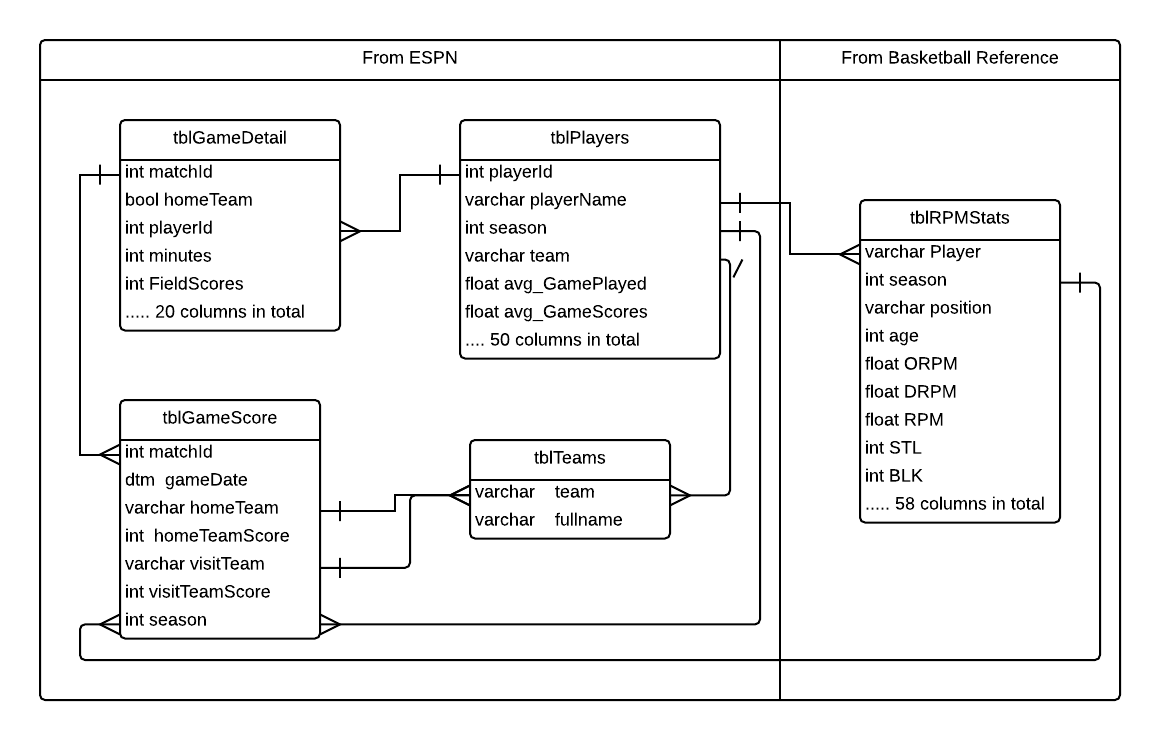
\includegraphics[width=150mm, height=150mm]{sqliteERDiagram.png}	
		\caption{Our database schema after merging the ESPN, Basketball Reference, and RAPM datasets together}
		\label{fig:database}
	\end{figure}

	%%% WEB CRAWLERS
	\subsection{Web Crawlers}
	To obtain all of these datasets, we used webcrawlers to pull them off their websites. All of these scripts can be found in our Github repository \cite{gitrepo}. For the ESPN data, we used the BeautifulSoup package in the Python language. For the other two datasets, we used the XML package in R. \\

	%%% TALK ABOUT MERGING SOURCES 
	\subsection{Merging Sources into One Database}
	One of the major obstacles in our project has been combining these three data sources into one single database. The ESPN dataset had both match and playerID's for each game, so merging the game statistics with the ESPN player database wasn't very difficult. However, the basketball reference and RAPM datset didn't have these identifiers, so it was more challenging to put them together. We ended up using the player's name, team, and season to join both of these datasets together with ESPN. Some common problems we had were inconsistent spelling of names in different datsets, inconsistent team names, teams have changed cities, etc.. In the end, we were able to sync most of the idiosyncracies between the three datasets, which is important because we will have more interesting features than just box score statistics. That being said, we don't doubt that there will still be further cleaning to do, and we will deal with these situations as they arise. \\

	%%% TALK ABOUT SQLITE LOADING DATA INTO DATABASE
	We are using an SQLite database to store all of the tidied data. The design of this database follows the third normal form to ensure there's no redundancy, and the indices were built on frequently used keys to ensure the queries are fast. Figure \ref{fig:database} displays our database schema. 

\section{Experiments}
	%%% TWOFEATURE MATRICES/.. LARGE AND JUST RPM/PER
	\subsection{Training and test datasets}
	We have put a substantial amount of time into constructing our training and test datasets. So far we have created two, one of which is using defensive and offensive RAPM, and the other uses all of ESPN's player statistics. To create these datsets, we went through each match to find the players on each team, and merged these players statistics from the previous season with the match results in the current season. To form the RAPM matrix, we used each players average minutes pergame from the season before as weights to compute weighted offensive and defensive RAPM statistic for each team. Say there's n players on each team, each playing m minutes per game with and RAPM score r in the previous season. Then the formula for the players weights and team offensive RAPM is:

	\begin{align*}
		w_i &= \frac{m_i}{\frac{1}{n}\sum_{i=1}^{n} m_i} \\
		\text{Team Offensive RAPM} &= \frac{1}{n}\sum_{i=1}^{n} w_i \times r_i 
	\end{align*}

	%%% TABLE OF EXAMPLE MATRIX %%%
	\begin{table}[ht]
	\centering
	\begin{tabular}{rrrrrr}
	  \hline
		ORPM\_home & DRPM\_home & ORPM\_away & DRPM\_away & homeWin \\ 
	  \hline
		-0.28 & 0.89 & 0.65 & 0.18 & 1 \\ 
	  	-0.28 & 0.89 & 1.15 & 1.05 & 1 \\ 
	  	-0.29 & 0.99 & -1.44 & 0.12 & 1 \\ 
	  	 0.03 & -0.66 & 0.04 & 1.09 & 1 \\ 
	  	 0.28 & 1.26 & -0.81 & -0.20 & 0 \\ 
	  	-0.75 & -0.46 & 0.51 & 1.02 & 1 \\ 
	   \hline
	\end{tabular}
	\caption{A look at what our training and test datasets look like. The first four columns are features and the 5th column (indicating whether or not the home team won the game) is our label}
	\label{table:matrix}
	\end{table}

	%%% BOTH GIVE 67% ACURACY
	\subsection{Classification}
	After constructing these two matrices, we were able to run classification algorithms on them to test their prediction accuracy. Given the amount of time effort that went into creating the datasets, we didn't have a lot of time to experiment with different algorithms and feature combinations. However, we were able to fit a Naive Bayes classifier, trained on the 2009 season and tested on the 2010 season, which gave us 67\% accuracy. We think this is a good sign, and with more work on the specific algorithms and features we think we can achieve rates similar if not higher than those achieved before us.

	\begin{figure}[h]
	\centerline{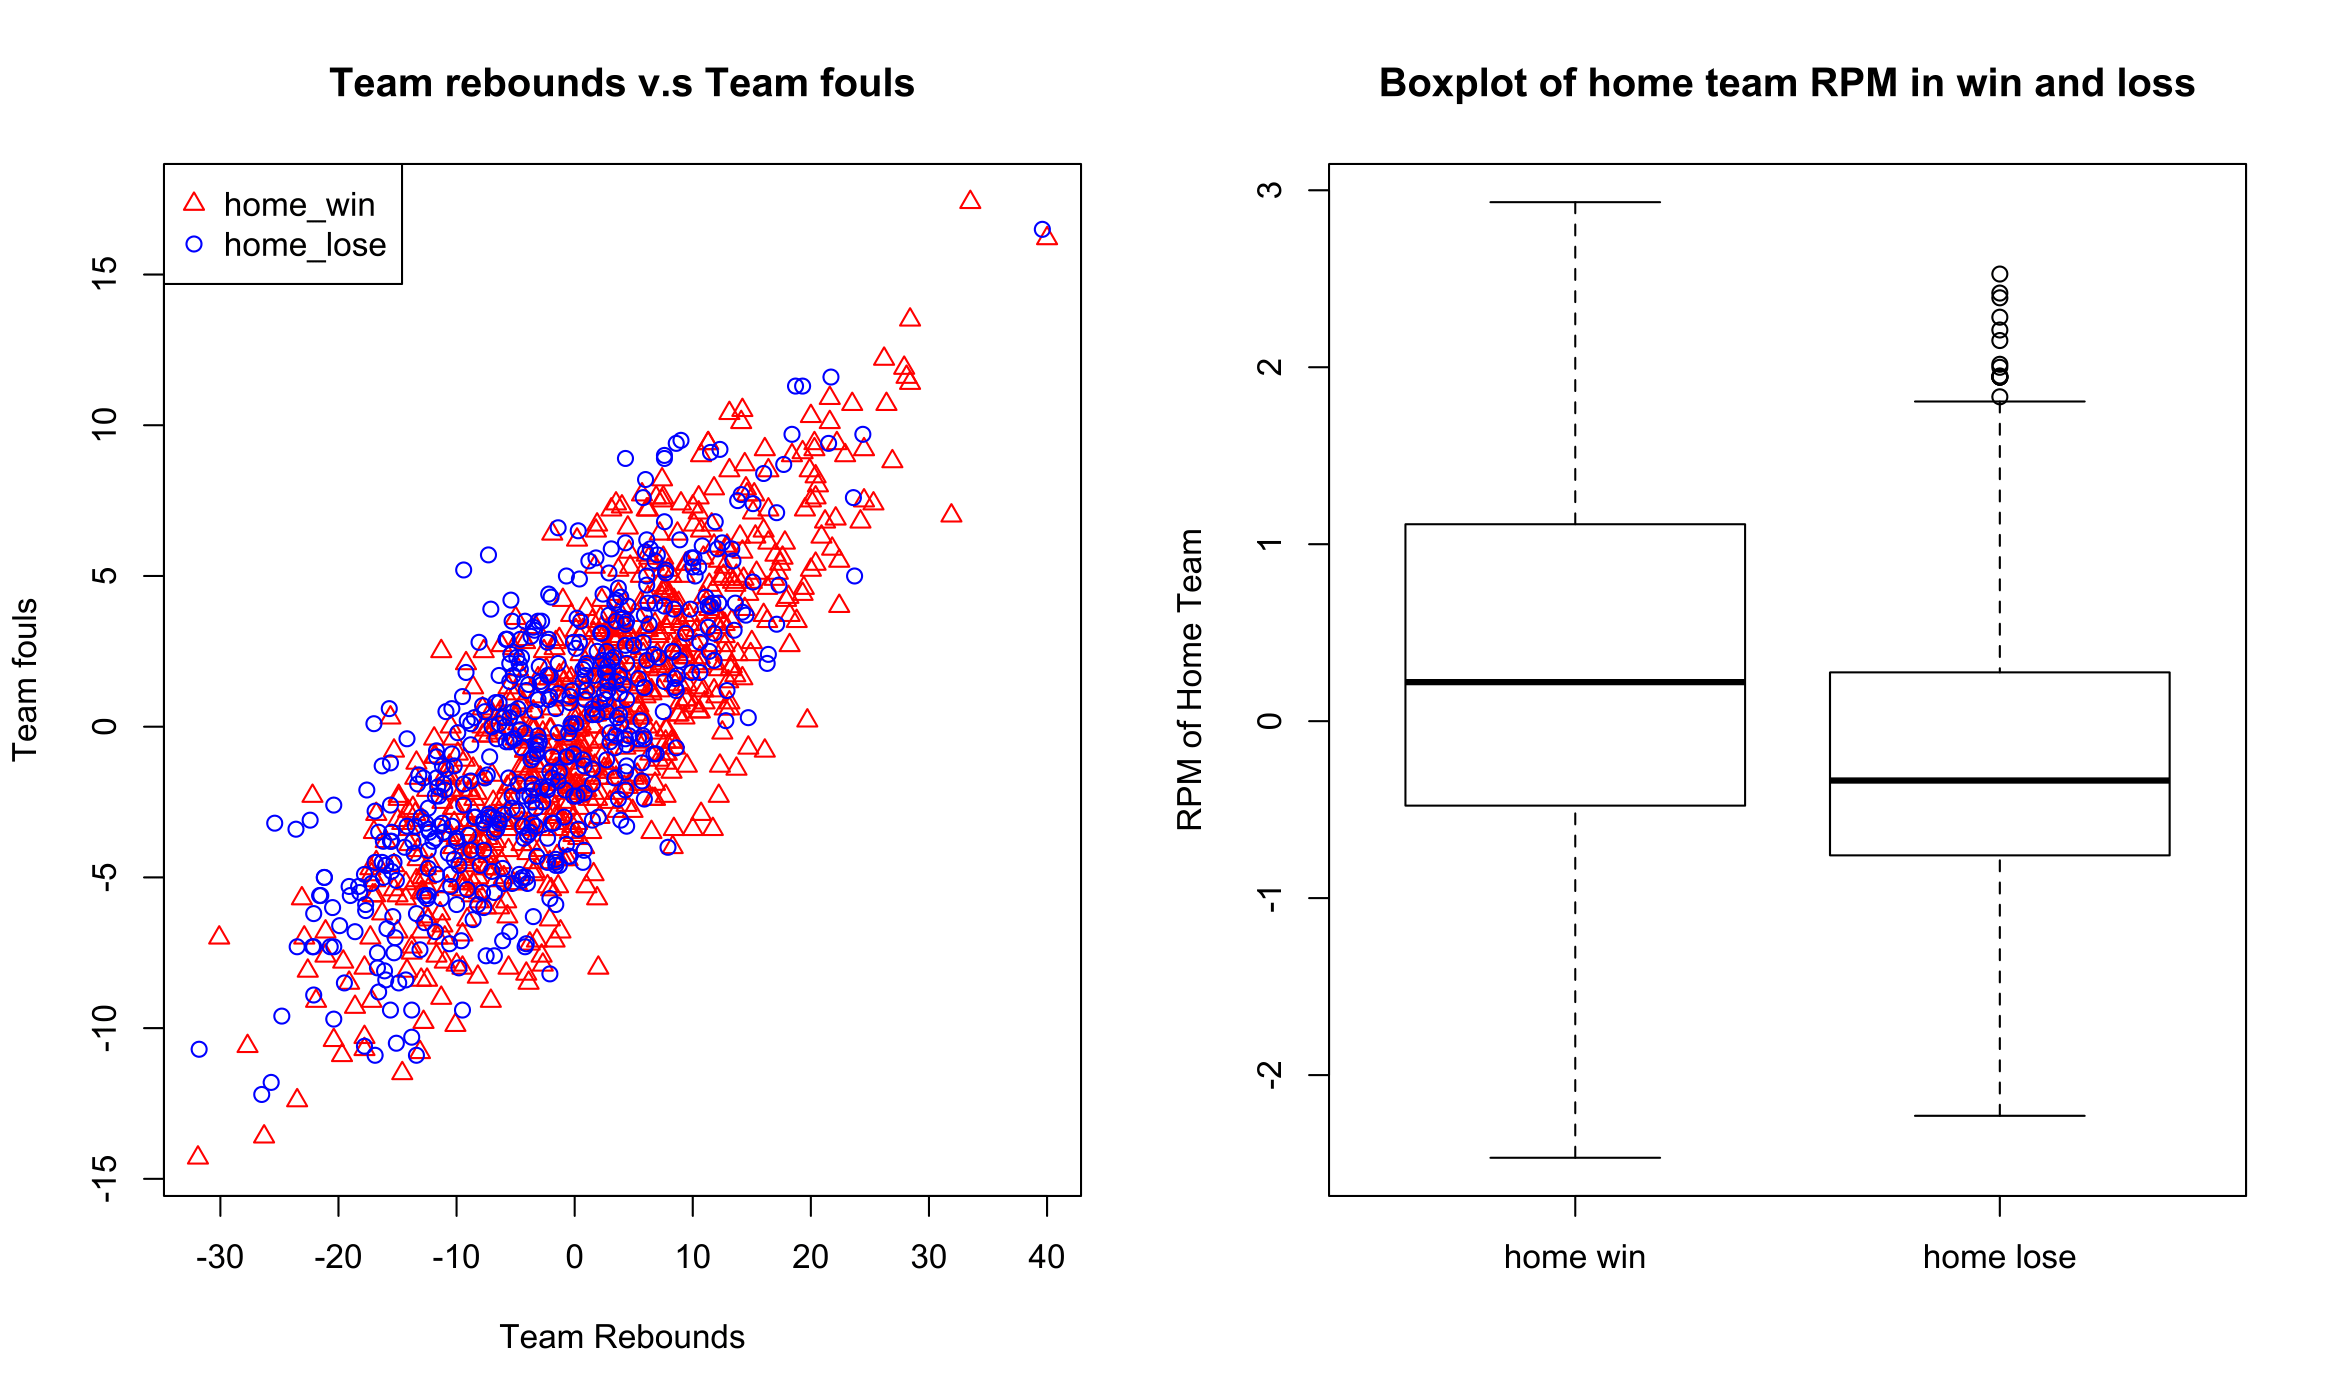
\epsfig{file=features.png, width=4.5in,height=3.25in}}
	\caption{On the left is a plot showing the correlation between two features in our dataset. This shows that our data is not linearly seperable for these two features, which is common among this dataset. However, we do see that there is some signal between wins and losses for these two features, as a higher score indicated a higher chance of winning the game. On the right, we look at team RAPM in wins compared with losses. As we can see, RAPM is clearly higher in wins than losses, so their is clear signals coming from this feature, as expected. }
	\label{feats}
	\end{figure} 

	\subsection{RPI}
	This sections borrows the idea of a team ranking method called the Rating Percentage Index (RPI), commonly used in college basketball. It is based on winning percentages; a team's RPI score is a weighted average of the winning percentages of teams, their opponents, and their opponents' opponents. To be more specific, we define $W,S\in \mathbb{R}^{n\times n}$,
	
	\begin{eqnarray}
	W_{ij}&=&\#\{\text{team i beat team j}\},\\
	S_{ij}&=&\sum_{\text{game between team i and j}}\frac{\#\text{points i scored on j}}{\text{total points in game}}.
	\end{eqnarray}

	Define the vectors $w,l,d \in \mathbb{R}^n$, 
	$$w=W\bold{1}, l=W^t\bold{1}, d=(W+W^t)\bold{1}.$$
	\par The vector elements $w_i$ (resp. $l_i$) is the number of games won (resp. lost) by team $i$. The vector $d_i$ is the number of games played by team $i$. Denote $D=diag(d)$. We will assume that each team has played in at least one game, implying $D$ is invertible. We analogously define the vectors $s,t\in \mathbb{R}^n$, 
	$$s=S\bold{1}, t=S^t\bold{1}$$
	\par Obviously, Winning Percentage is the simplest rating method, and it can be easily computed as
	$$\Phi^{WP}=D^{-1}s$$
	where $\Phi_i^{WP}$ is the team $i$'s rating. This rating does not take into account the team's "strength of schedule". That is, a team is able to have a large winning percentage by playing poor teams. This is why the RPI was introduced, and it is computed as following,
	$$\Phi^{RPI}=\frac{1}{4}\Phi^{WP}+\frac{1}{2}D^{-1}(W+W^t)\Phi^{WP}+\frac{1}{4}(D^{-1}(W+W^t))^2\Phi^{WP},$$
	where $D^{-1}(W+W^t)\Phi^{WP}$ is the vector of average opponent's winning percentages and $(D^{-1}(W+W^t))^2\Phi^{WP}$ is the vector of average opponent's opponent's winning percentages. \\

	\begin{figure}[h]
	\centerline{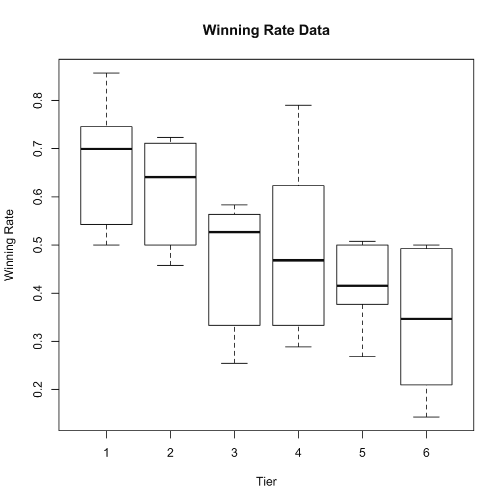
\epsfig{file=WinningRate2011.png, width=4.5in,height=3.25in}}
	\caption{Box Plot using 2011 to train the ranking and testing on 2012}
	\label{f1}
	\end{figure} 

	Our strategy is to use RPI to calculate teams' ranking in previous year, and compare it with teams' winning percentages in the following year.	In particular, since the number of games played between two teams are relatively small each year, we divide the ranking in six tiers where $tier1$ contains the top five teams, $tier2$ contains next best five teams, and so on. Then we compute the winning percentages of the games played between two tiers in the following year. Figure \ref{f1} indicates that the team which had RPI ranking in the previous year generally performs better in the following year. This suggests that we could use RPI ranking as a feature in our training process, which might improve the accuracy of our classifier.

\section{Future Work and Goals}

	\subsection{Realistic Goals}
	%% Play with different algorithms/feature datasets
	As mentioned above, a substantial amount of time was put into collecting and tidying the data, and creating usable datasets. Now that this has been completed, we have more time to focus on different classification algorithms and combinations of features, to see if we can improve our accuracy. Specifically, we hope to implement:

	\begin{itemize}
		\item Linear Regression
		\item Logistic Regression
		\item Support Vector Machine
	\end{itemize}

	%% ACHIEVE > 70 % TEST ERROR FOR ONE ON OUR SEASONS
	We believe it is a realistic goal to achieve a 70\% classification rate on one of our seasons before the end of the course. 

	\subsection{Missing data and Outliers}
	One of our goals is to come up with better methods for handling missing data. We already have a fairly clean data frame. However due to different reasons we still have some missing points in our dataset. We typically use the league average to fill in missing datapoints for our features. For example, since RAPM has an average of 0 by definition, we automatically give a player a score of 0 if his score is missing for a given season. As we see in figure \ref{feats}, there's some data that are pretty far from the average, which are potentially outliers. For example, when a team clinches the playoffs at the end of a season, they may not play all of their starters, which result in features with much larger variances, since the players being used don't typically play a lot of minutes. We will closely inspect our dataset for outlier. If/when we find questionable datapoints, we will investigate individual cases to see if they were due to data error or if they are real values, and take action accordingly. 

	\subsection{Stretch Goals}
	%%% not just past year, past 3 years or projections 
	One part of our classification that could be improved is that we are only using the previous seasons data to predict the current season outcomes. There are some obvious issues with this strategy. For instance, some rookies, even if they're productive (or horrible) players, don't have statistics from last season, so we are just assigning them league average rates. Also, some players, for example former MVP Derrick Rose, was injured for an entire season, so using just the last year to predict a game and discounting his MVP season would misrepresent the quality of the Chicago Bulls. To combat these issues, we think it may be helpful to use more than just last seasons data, perhaps using the average of the last three years, or set up a projection system. The first seems like a more tractable goal than actually making projections, which could probably spawn an entirely new project. \\

	One other method we could use to improve our accuracy is to use games from the current season which have already happened. To do this, we can chop our season into subsets and order them by the time they were played. Then, we can use the team win percentages in all of the games before the one being predicted as a feature in our classification. That way, we should be able to predict games later in the season more accurately that games earlier in the season. \\
		
	% simulating the whole season, using game probabilities and picking U(0,1) multiple runs through the season to ge distributions of wins. 
	Another thing we've thought about trying is predicting the number of wins for each team in a season, as opposed to just single game results. To accomplish this, consider fitting a Naive Bayes model. The outcome is two probabilities of each team winning the game, and in prediction we just take the maximum. We could compress these probabilities to sum up to one, and then use a $\sim$ Uniform(0,1) random variable to decide the winner of each game. We could do this for each game in the season and add up the wins and losses for each team. Then we could repeat this process a few thousand times to generate a distribution of total wins for each team, and compare these with the actual number of wins in a season.

%%%%%%%%%%%%%%%%%%%%%%%%%%%%%%%%%%%%
%%%%%%%%%% BIBLIOGRAPHY %%%%%%%%%%%%
%%%%%%%%%%%%%%%%%%%%%%%%%%%%%%%%%%%% 
 
  \begin{thebibliography}{1}

  \bibitem{nba_oracle} Matthew Beckler, Hongfei Wang, Michael Papamichael {\em NBA Oracle} 2009.

  \bibitem{data_mining} Dragan Miljkovic, Ljubiša Gajic, Aleksandar Kovacevic, Zora Konjovic {\em The Use of Data Mining for Basketball Matches
Outcomes Prediction} 2010: SISY 2010

  \bibitem{rpm} Paul Fearnhead, Benjamin M. Taylor {\em On Estimating the Ability of NBA Players}. 2010: http://arxiv.org/pdf/1008.0705.pdf.

  \bibitem{bigrpm} Steve Illardi. {\em The next big thing: real plus minus}. 2014. ESPN.com

  \bibitem{rpm_data} Jeremias Engleman. http://stats-for-the-nba.appspot.com/

  \bibitem{bball_ref} Basketball Reference. http://www.basketball-reference.com/

  \bibitem{espn} ESPN. http://espn.go.com/nba/.

  \bibitem{gitrepo} Repository for Game Simulation. https://github.com/leerichardson/game\_simulation.

  \end{thebibliography}

\end{document}	